%!TeX root=../tese.tex
%("dica" para o editor de texto: este arquivo é parte de um documento maior)
% para saber mais: https://tex.stackexchange.com/q/78101

% Aqui podemos começar falando um pouco sobre o background de explainable AI e depois conectamos
% falando sobre redes neurais e gradiente descendente para, por fim, falar um pouco sobre CNNs.


\enlargethispage{-1\baselineskip}

\chapter{Background}

In this chapter, we will introduce important concepts required for the understanding of this study.
We begin by introducing Explainable AI (XAI) and its principles. We also introduce Neural Networks and important concepts such as Gradient Descent and Back Propagation. 
Finally, we introduce Convolutional Neural Networks, the main focus of this study.

\section{Explainable AI}

With the rise of Machine Learning models in the last decade in the business and academic areas, Artificial Intelligence (AI) is becoming increasingly present in important decision-making tasks. 
However, as AI models have become more sophisticated, particularly with the advent of Deep Learning techniques, their internal workings have often remained opaque. 
Explainable AI (XAI) aims to make models and their decisions more transparent, interpretable and understandable to both experts and inexperienced users.

\subsection{What is Explainable AI?}

Defining a mathematical formalization to explainability of Machine Learning is a difficult task considering the subjective nature of what one may consider "explainable". In non-mathematical terms, 
Explainability in AI refers to the capacity to articulate or justify the behavior of a model, focusing on methods that explain a model's decisions after they are made.

Another important concept in the area is Interpretability, which can be defined as "the degree to which a human can understand the cause of a decision" by Miller (2017)\footnote[1]{Miller, Tim. “Explanation in artificial intelligence: Insights from the social sciences.” arXiv Preprint arXiv:1706.07269. (2017).}.
In this case, however, a model's decision is understandable entirely by its inherent transparency. In other terms, the model is simple enough to be interpretable by a human directly, without the use of external techniques.

Models with low complexity whose decisions are understandable by humans are defined as \emph{Interpretable Models}. Linear Regression, Logistic Regression and Decision Tree models are examples of models classified as \emph{Interpretable Models}. 
Now, models with a level of complexity that prevents humans from directly understanding their decision-making processes are referred to as \emph{Explainable Models}. 
Recently popular \emph{Deep Learning Models} are one kind of \emph{Explainable Models} and will be the main focus of this essay, especially \emph{Deep Convolutional Neural Networks}, explored in \hyperref[sec:convolutions]{section 1.3}.
% CUIDADO AQUI EM CIMA!!! PODE MUDAR O NÚMERO DA SESSÃO

\subsection{Why Explainable AI is Necessary}

Creating explanations to a model's decisions can yield many advantages, including  more ethical and fair decisions, correctly following regulatory compliances and easier model debugging.

To ensure ethical and fair decision-making, Machine Learning systems must provide justifiable decisions, as they often exploit discriminatory patterns to enhance accuracy, which can perpetuate harmful biases. 
For instance, the COMPAS algorithm, used in U.S. courts to assess recidivism risk, was analyzed by ProPublica\footnotemark and found to exhibit significant bias against Black defendants, frequently overestimating their likelihood of reoffending compared to their actual risk.
\footnotetext{\emph{"How We Analyzed the COMPAS Recidivism Algorithm", by ProPublica: https://www.propublica.org/article/how-we-analyzed-the-compas-recidivism-algorithm}}

Explainable AI (XAI) is sometimes a mandatory requirement, particularly under regulations like the United Kingdom's General Data Protection Regulation (GDPR). 
The GDPR mandates that organizations must provide clear and understandable explanations for decisions that significantly impact individuals, especially those made by automated systems commonly powered by Machine Learning algorithms. 
Without XAI, high-stakes decisions cannot leverage such models in the United Kingdom, highlighting the crucial role of explainability in enabling the broader adoption of Machine Learning for real-world applications while ensuring compliance and fairness.

When debugging Machine Learning models, their behavior can often be unpredictable, revealing biases that may not have been initially apparent to humans. 
These biases can result in high performance on training, validation, or even test datasets but lead to poor performance in real-world deployment. 
For instance, consider training an image classifier to differentiate between dog and cat images. 
The model may achieve impressive accuracy on images of dogs in green fields. 
However, upon examining the regions of the image the model relies on for its predictions, researchers might discover that it focuses on the background rather than the animals themselves. 
This happens because dog owners are more likely to photograph their pets outdoors, leading to an unintended association between dogs and green backgrounds. 
Techniques from Explainable AI, such as Grad-CAM \citep{Selvaraju_2019} and Gradient Saliency methods, enable researchers to visualize these image regions, providing critical insights into model behavior and helping to address such biases.

\section{Gradient Descent}
\label{sec:gradient_descent}

Let \(f\colon A \to B\) where \(A \subseteq \mathbb{R}^n\) for \(n \in \mathbb{N}\) and \(B \subseteq \mathbb{R^+}\). Suppose we want to find the solution to the optimization problem

\begin{equation}
    \argmin_{x \in A} f(x)
    \label{eq:min_func}
\end{equation}

when \(\frac{\partial f}{\partial x}\) is known for any value of \(x\). Considering that the vector \(\frac{\partial f}{\partial x}\) points to the direction of the steepest ascent of the function, the vector \(- \frac{\partial f}{\partial x}\) will point to the steepest descent from the given point \(x\).
Therefore, one can define an initial random value for \(x\) and update \(x\) using \(- \frac{\partial f}{\partial x}\) and a scaling factor \(\eta\) in order to find a local minimum of \(f\) and an approximation to the solution of given optimization problem.

We can define such method using the following formula, where \(x_t\) represents the value of \(x\) at iteration \(t\) of the algorithm:

\begin{equation}
    x_{t + 1} = x_t - \eta \frac{\partial f (x_t)}{\partial x_t}.
    \label{eq:gradient_descent}  
\end{equation}

The term \(\eta\) is often called the \emph{learning rate} used in the Gradient Descent method and is often defined manually by the user.

The Gradient Descent method can be used to optimize a neural network's parameters to solve a given problem using a \emph{loss function}. 

\section{Neural Networks}

Neural Networks are proven to be universal approximators\footnote{Hornik, K., Stinchcombe, M., White, H. Multilayer feedforward networks are universal approximators. https://doi.org/10.1016/0893-6080(89)90020-8}. That means that Neural Networks are Machine Learning models capable of representing any continuous function,
therefore making Neural networks adept at modeling a range of different complex problems.
This class of models have seen a growing presence across both academic and industry landscapes. However, given the architecture of multiple hidden layers of Neural Networks creating complex internal patterns, such models are classified as Explainable Models. 

In this section, the inner workings of Neural Networks will be explained, starting with the \emph{Perceptron}, considered the fundamental building block of Neural Networks.

\subsection{Perceptron}

A Perceptron is a Machine Learning model inspired by how biological neurons work. 
It is a simple binary linear classifier that defines its parameters by linear combinations of points in the dataset.
The Perceptron model can be described by Figure \ref{fig:perceptron}. 

\begin{figure}
    \centering
    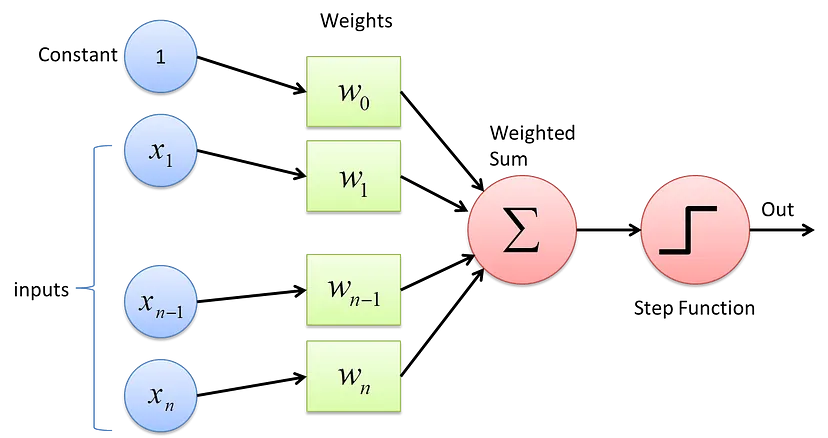
\includegraphics[scale=0.4]{figuras/perceptron.png}
    \caption{Perceptron Architecture. Font: \emph{Towards Data Science\footnotemark}. \label{fig:perceptron}}
\end{figure}
\footnotetext{https://towardsdatascience.com/what-the-hell-is-perceptron-626217814f53}

Where the weights \(w_i\) for \(i \in \{0, 1, \cdots, n\}\) are trainable parameters and the step function can be defined as \(\sigma \colon \mathbb{R} \to \{0, 1\}\) such that

\begin{equation}
    \sigma(x) = 
    \begin{cases}
        1 & \text{ if } x \geq 0 \\
        0 & \text{ if } x < 0.
    \end{cases}
    \label{eq:step_function_perceptron}    
\end{equation}

Therefore, the Perceptron model can be defined as the function\footnotemark \(f \colon \mathbb{R}^n \to \{0, 1\}\) where
\footnotetext{The independent term \(w_0\) is usually called the \emph{bias} of the Perceptron (or neuron)}
\begin{equation}
    f(x) = \sigma(w_0 + \sum_{i = 1}^{n} w_i x_i).
    \label{eq:perceptron}
\end{equation}

The Perceptron model updates its parameters using each sample \((x, y)\) of the dataset with the rule

\begin{equation}
    w_i^{t + 1} = w_i^t + \eta \; (y - f(x)) x_i
    \label{eq:perceptron_update}  
\end{equation}

\noindent for \(i \in \{1, \cdots, n\}\) and

\begin{equation}
    w_0^{t + 1} = w_0^t + \eta \; (y - f(x)),  
\end{equation}

\noindent where \(\eta\) is the \emph{learning rate} hyperparameter and \(t\) is the update iteration number.

As a linear model, the Perceptron can only model linear problems, which only represent a small subset of real world problems.
As a solution, researchers started combining Perceptrons in a layered structure, called Multilayer Perceptron, also famously known as \emph{Neural Networks}.

\subsection{Multilayer Perceptron (MLP)}

By stacking multiple Perceptrons into multiple layers, one can build more complex decision boundaries and model more complex functions. 
For example, by using the Multilayer Perceptron, one can model a XOR function: 

\begin{figure}
    \centering
    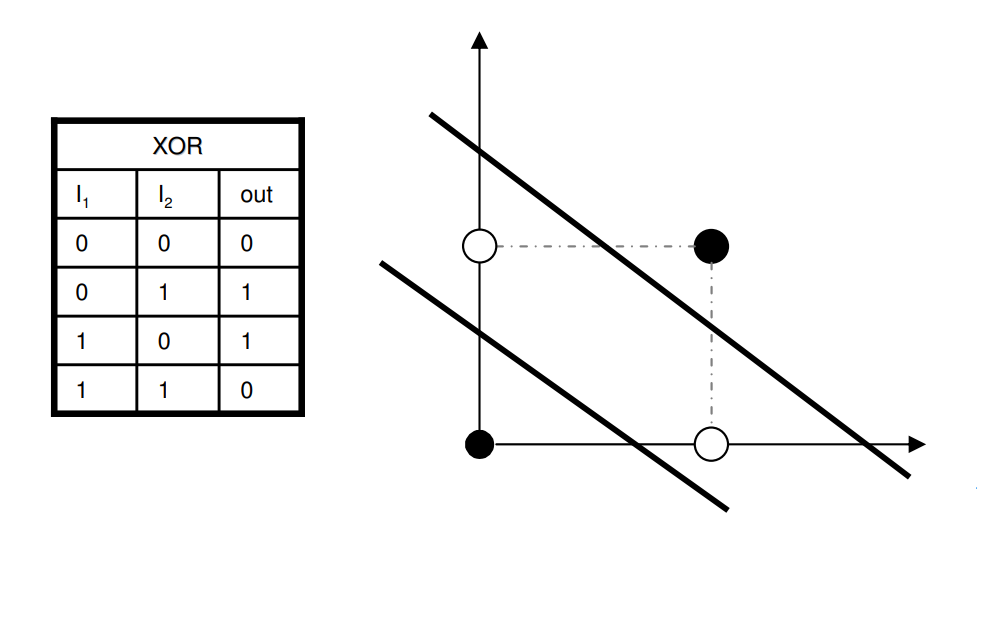
\includegraphics[scale=0.4]{figuras/xor_problem.png}
    \caption{The XOR Problem Font: \emph{Kevin Swingler Lecture Notes}. \label{fig:xor_problem}}
\end{figure}

The XOR problem can not be solved by using a single Perceptron, since it is not a linear problem.
However, by using two Perceptrons (which corresponds to the two lines in the figure), one can model the non-linear XOR problem.  
In this specific example, one can define the uppermost line as the decision boundary of the Perceptron \(f_1(x) = \sigma(- x_1 - x_2 + 1.5)\) and the lowermost line as the decision boundary of the Perceptron \(f_2(x) = \sigma(x_1 + x_2 - 0.5)\).
Considering the Perceptrons \(f_1\) and \(f_2\), we can create a new Perceptron that receives the outputs of those Perceptrons and returns the result of the XOR function. 
For example, we can define the Perceptron \(g(x) = \sigma(x_1 + x_2 - 1.5)\), generating the following results:
\begin{table}[h!]
    \centering
    \begin{tabular}{|c|c|c|c|c|}
    \hline
    $x_1$ & $x_2$ & $f_1(x)$ & $f_2(x)$ & $g(f_1(x), f_2(x))$ \\ \hline
    0     & 0     & 1     & 0     & 0   \\ \hline
    0     & 1     & 1     & 1     & 1   \\ \hline
    1     & 0     & 1     & 1     & 1   \\ \hline
    1     & 1     & 0     & 1     & 0   \\ \hline
    \end{tabular}
    \caption{Perceptron output for binary combinations of \(x_1\) and \(x_2\).}
    \label{tab:xor_table}
\end{table}

\noindent Showing that the non-linear problem can be successfully be solved by the Multilayer Perceptron.

Although the Multilayer Perceptron has the perk of being able to model complex functions, we are still limited by how to model is trained, since it cannot be trained by using the update rule of the traditional Perceptron.

By using a technique known as Backpropagation, the Multilayer Perceptron can be trained using gradient-based update rules, like the Gradient Descent.

\subsection{Backpropagation}

In order to find the weight's gradients of our MLP, one can use Backpropagation, a technique that involves computing those gradients by performing a \emph{Forward Pass} and a \emph{Backward Pass} on the Neural Network.

\subsubsection{Forward Pass}

The Forward Pass basically consists in computing the input through the network and comparing the output with the expected value using a loss function \(\mathcal{L}\).
During the forward pass, the output of each layer is stored in memory to be later used in the Backward Pass.

\subsubsection{Backward Pass}

In the Backward Pass, the gradients of the loss with respect to the weights are calculated to update the network. 
By using the chain rule, one can start off by calculating the gradients of the last layer of the network, and then use the result to calculate the gradients of the weights of the previous layer, \emph{going on the opposite direction of the Forward Pass}.

\subsubsection{Updating Weights}

With the gradients of the loss with respect to the weights calculated, now the weights are updated in an iterative process, until a satisfiable loss/accuracy is achieved or new model/dataset tunning is necessary. 

\section{Convolutional Neural Networks}
\label{sec:convolutions}
\subsection{Convolutions}
First, it is important to define what a convolution is. Given two discrete one-dimensional signals \(f\) and \(g\), their convolution \(f * g\) is defined as:
\[
(f*g)[n] = \sum_{i=-\infty}^{+\infty} f[n] g[n-i]
\]

Given two discrete two-dimensional signals \(f\) and \(g\), their convolution \(f * g\) is calculated as:

\[
(f*g)[m][n] = \sum_{i=-\infty}^{+\infty} \sum_{j=-\infty}^{+\infty} f[m][n] \cdot g[m-i][n-j]
\]

In practice, the signal \(g\) is represented by a window (or kernel), usually square and of odd size. Thus, we can abstract convolution as the multiplication of a sliding window. The picture below illustrates this process. It is important to note that the window needs to be flipped during the convolution, although this is not illustrated in the picture.

\begin{figure}[h!]
    \centering
    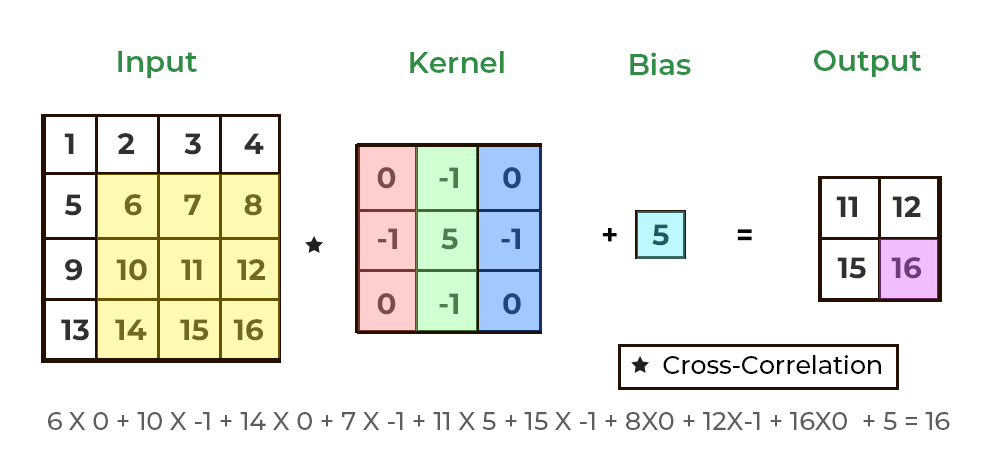
\includegraphics[width=0.5\textwidth]{figuras/conv.png}
    \caption{2D Convolution}
\end{figure}

This process can be used to apply different filters to images. For example: using a \(3 \times 3\) window with all weights equal to \(\frac{1}{9}\), we can generate a filter that blurs the image (moving average). Below is an example of applying this filter:

\begin{figure}[h!]
    \centering
    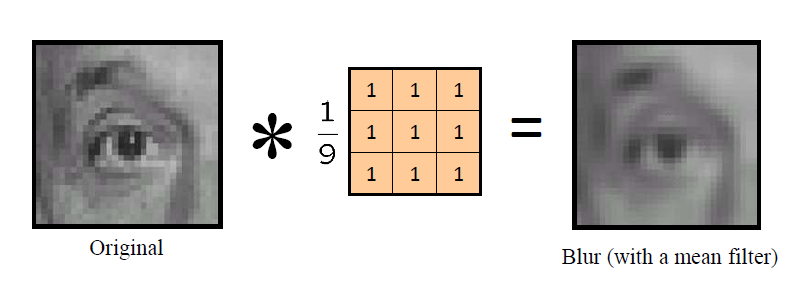
\includegraphics[width=0.5\textwidth]{figuras/blur.png}
    \caption{Filtered Image (3x3 Mean Filter)}
\end{figure}

It is also important to note that convolution is commonly implemented in machine learning contexts as "cross-correlation," which is a very similar operation but without the flipping of the window. Note that, since the weights are learned in our case, there is no difference. Therefore, in our context, convolution and cross-correlation are synonymous.

\begin{figure}[h!]
    \centering
    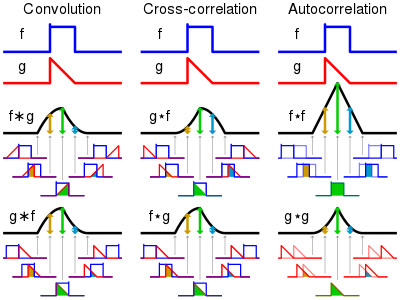
\includegraphics[width=0.5\textwidth]{figuras/cross-correlation.png}
    \caption{Comparison with Cross-Correlation}
\end{figure}

A pertinent question that can be asked is what happens at the edges of the image. When the window is sliding over them, what happens to the missing pixels? The process of filling in these pixels is called padding. Padding can be done with zeros, the nearest pixel, or not be done at all. Note that when there is no padding, the image decreases in size after convolution.

Another important hyperparameter that can be adjusted is the "stride." This defines how many positions the window is moved at a time. That is: a stride value different from 1 also implies a decrease in image size after convolution.

\subsection{Convolutional Layer}

In order to understand the need for convolutional networks, we have to understand why it's impractical to use fully-connected networks to process images. Let's walk though an example to see that. 

Consider a color image with dimensions 512x512. If we were to process this image with a conventional neural network, the input layer would have \( 3 \cdot 512 \cdot 512 = 786432 \) dimensions. Assume a hidden layer with only 128 neurons (which is relatively small). Just between these two layers, there would be \( 100663296 \) parameters! This is highly inefficient.

The solution to this problem is to extract features from the image, which will serve as input to the network. These features could include various aspects such as symmetry, black levels, contrast, presence or absence of patterns, etc. All of these features will serve as input to the network. As a result, we can reduce the input layer's dimensionality from several hundred thousand to just a few dozen.


However, a challenge still remains: how do we select these features? We can apply convolutions to the image to calculate interesting features, and these convolutions can be learned alongside the rest of the network! It is important to understand some essential details about these networks before proceeding. Each convolutional layer has three dimensions: height, width, and the number of channels. The input layer typically has one channel for black and white images, or three channels for color images.

Each channel in each convolutional layer combines all the channels from the previous layer. In other words, the "windows" used have weights for all the channels. These windows slide over the data from the previous layer to generate \textbf{one channel} in the next layer.

Let us consider an example. Suppose we have a network that processes color images of size \( 128 \times 128 \) pixels. This network has 3 convolutional layers with 16, 32, and 64 channels per layer, respectively. Assume a window size of 3 for all layers. In this case, we have:

\begin{itemize}
    \item First layer: window size is \( 3 \times 3 \times 3 \). With 16 output channels, we will have 
    \[
    16 \cdot 3 \cdot 3 \cdot 3 = 432 \text{ parameters.}
    \]
    \item Second layer: window size is \( 3 \times 3 \times 16 \). With 32 output channels, we will have 
    \[
    32 \cdot 3 \cdot 3 \cdot 16 = 4608 \text{ parameters.}
    \]
    \item Third layer: window size is \( 3 \times 3 \times 32 \). With 64 output channels, we will have 
    \[
    64 \cdot 3 \cdot 3 \cdot 32 = 18432 \text{ parameters.}
    \]
\end{itemize}


Another important detail is the output dimension of each layer. This depends on whether or not \textbf{padding} is used. \textbf{Padding} refers to how the layer behaves at the image edges. We can complete the image with zeros, the nearest pixel value, or the pixel value from the opposite edge of the image. If padding is not used, the output dimensions will decrease by \( 2 \lfloor \frac{W}{2} \rfloor \), where \( W \) is the window size. For instance, with a window size of 3, each layer will reduce the image size by 2 pixels. If the input is \( 128 \times 128 \), the output of the first layer will be \( 126 \times 126 \), the second layer will output \( 124 \times 124 \), and so on.

\subsection{Pooling}

Remember, each convolution extracts a feature from the image. Therefore, when we perform another convolution using the outputs from the previous layer, we are combining features extracted from the image to compute new features. As a result, deeper layers extract more complex features from the image. For instance, the first layer may extract features like the presence of vertical straight lines, while the tenth layer may extract features like "presence of dog snouts."

Thus, the features involved gradually become less localized and more global (pertaining to the entire image). This is why it is useful to summarize information into smaller dimensions as the network deepens.

To accomplish this, we use "pooling" layers. These layers work similarly to convolutions: windows slide over the data and compute an output based on nearby pixels. However, this time, a function is used to aggregate these data. Common functions include "max" (maximum value) and "avg" (average value).

\begin{center}
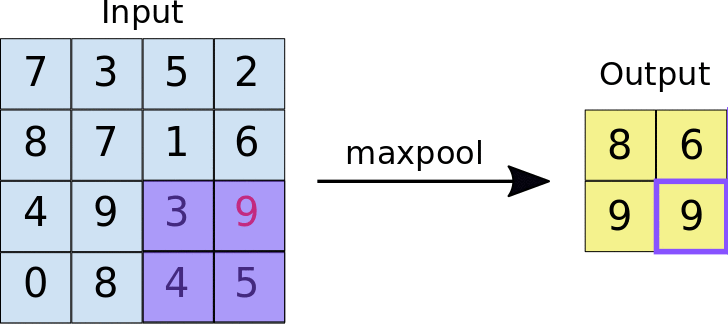
\includegraphics[width=0.8\textwidth]{figuras/max_pool.png}
\end{center}

\subsection{Receptive Field}

An important concept for understanding the power of \textbf{deep convolutional networks} is the \textbf{receptive field}. This concept relates to the power that chained convolutions have.

Consider an input image. Apply a \( 3 \times 3 \) convolution to it. Now, apply another \( 3 \times 3 \) convolution to the output of the first convolution. Observe this output image. How much information does each pixel contain about its neighbors?

\begin{center}
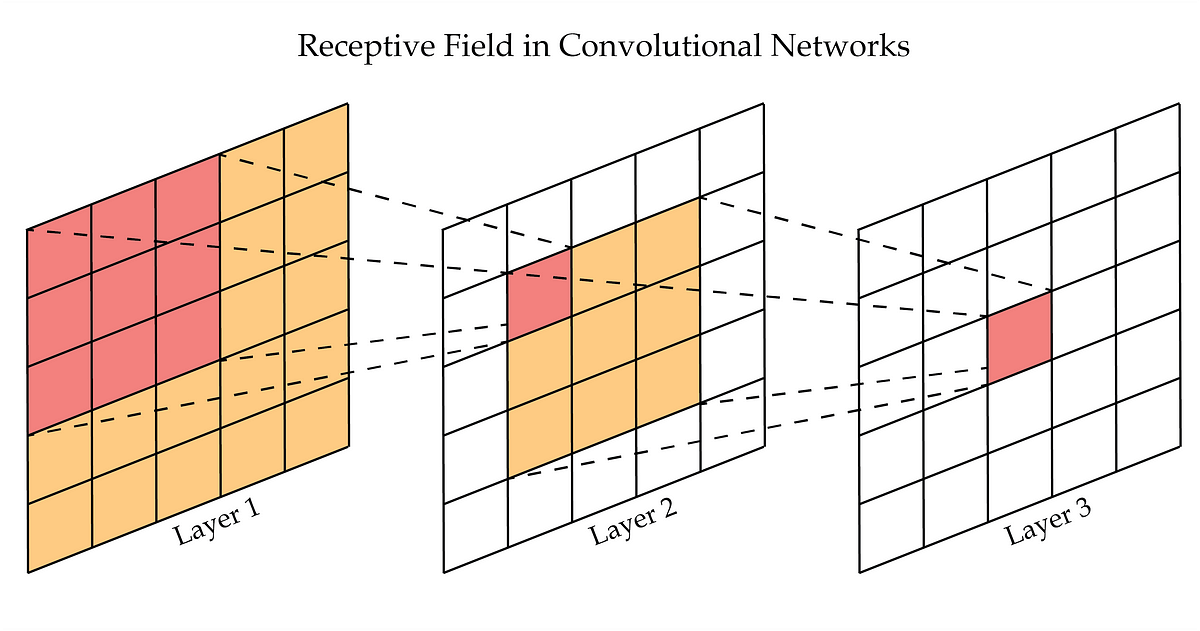
\includegraphics[width=0.8\textwidth]{figuras/receptive_field.png}
\end{center}

The answer is that each pixel contains information from a region of size \( 5 \times 5 \) around it! This is the receptive field of these neurons.

A common misconception is that, since the receptive field of two \( 3 \times 3 \) convolutions is \( 5 \times 5 \), two \( 3 \times 3 \) convolutions have the same \textbf{expressive power} as a \( 5 \times 5 \) convolution. This \textbf{is not} true. A \( 5 \times 5 \) convolution has 25 parameters, while two chained \( 3 \times 3 \) convolutions only have 18 parameters.





